\chapter{Communication Strategies}
In parallel implementations of SpMV, effective communication management is critical due to its significant influence on overall performance. Communication often emerges as a bottleneck in distributed-memory systems because the speed at which data moves between nodes is significantly lower than within-node memory access speeds. Consequently, reducing communication volume and optimizing communication patterns can yield substantial performance improvements.
\medskip

This chapter evaluates a series of progressively optimized communication strategies employed in distributed-memory parallel SpMV. Starting from the simplest method, exchanging the entire result vector between all nodes, the strategies become increasingly selective and efficient, focusing specifically on exchanging only the essential data elements required by each node. Finally, a communication strategy that is fully memory scalable is described. These approaches leverage knowledge of the matrix structure, partitioning methods, and computational dependencies to minimize communication overhead.
\medskip

In the subsequent sections, each figure illustrating a communication strategy is based on the graph shown in Figure \ref{fig:examplegraph} as an example of a partitioned graph. In this example, each colour denotes the rank assigned to the vertices contained in the corresponding partition.

\begin{figure}[H]
    \centering
    \incfig{examplegraph}
    \caption{Simple graph partitioned amongst rank - each color represents a rank.}
    \label{fig:examplegraph}
\end{figure}

\section{Strategy A - Exchange entire vector}
In this strategy, at each iteration every rank sends its locally computed values of \(y\) to all other ranks so that each process obtains a complete copy of the output vector before proceeding. This approach can be implemented with the MPI collective operation \texttt{MPI\_Allgatherv}, which supports different send and receive counts on each rank. \autoref{alg:1acomm} shows how this communication pattern can be implemented.
\medskip

\begin{algorithm}[H]
    \label{alg:1acomm}
    \caption{Strategy A - Communication Pattern}
    \SetAlgoVlined
    \For{each iteration}{
        spmv(g,x,y)\\
        MPI\_Allgatherv(local\_y, sendcount, MPI\_DOUBLE, y, recvcounts, displs, MPI\_DOUBLE, MPI\_COMM\_WORLD)\\
        swap pointers of \(x\) and \(y\)
    }
\end{algorithm}
\medskip

Let \(n_{p}\) denote the total number of ranks, and let \(\left| x_{i} \right|\) be the number of vector entries assigned to rank \(i\) (given by the average; \(\frac{\left| x \right|}{n_{p}}\)). Since each rank must send its local block size of \(\left| x_{i} \right|\) to the other \(n_{p}-1\) ranks, the total volume of communication per iteration is given by \ref{eq:1a}.

% Let \(n_{p}\) denote the total number of ranks, and \(\left| x \right|\) be the size of the vector \(x\). Since each rank must send each vector entry it is assigned to each, the total communication volume is given by

\begin{equation}
    \label{eq:1a}
    \text{Total Communication} = n_{p} \cdot  (n_{p}-1) \cdot \left| x_{i} \right|
\end{equation}

Figure \ref{fig:1acomm} illustrates the state of the vector before and after communication using this strategy.

\begin{figure}[H]
    \centering
    \incfig{1acomm-2}
    \caption{Contents of each ranks vector before and after communication under the \textit{Exchange Entire Vector} communication pattern.}
    \label{fig:1acomm}
\end{figure}

\section{Strategy B - Exchange only separators}
An improvement to the previous strategy can be achieved by recognizing that only separator values, those required by multiple processes, must be communicated. Non-separator values are used exclusively by the process that computed them and therefore do not need to be communicated. 
\medskip

Let \(n_{p}\) denote the total number of ranks, and let \(s_{i}\) be the size of the separator of rank \(i\). Since each rank sends its separator to each other rank (i.e. \(n_{p} - 1 other ranks\)), then the total communication volume is given by \ref{eq:1bcomm}.

\begin{equation}
    \label{eq:1bcomm}
    \sum_{i=1}^{n_{p}}(n_{p} - 1) \cdot s_{i} 
\end{equation}

To facilitate this strategy, separator values are reordered such that they appear at the beginning of each process's local segment of \(y\). Once this structure is established, communication is performed using \texttt{MPI\_Allgatherv}, transmitting only the subset of \(y\) that contains separator values. The number of separators on each process must be known beforehand, which can be computed by counting the number of elements that have neighbours belonging to a different partition.

\subsection{Reordering}
After partitioning the matrix into different parts, we obtain a partition vector \(p\), where the \(p[i]\) stores the index of the partition the \(i^{\text{th}}\) entry in \(A_{p}\). It is necessary to reorder the entries in \(A_{p}\) in accordance with the partition vector, such that all entries belonging to the same partition are stored in sequence. The algorithm below gives an outline of how this can be achieved. Here \(n_{p}\) is the number of partitions, \(n_{r}\) is the size of \(A_{p}\), and \(n_{c}\) is the size of \(A_{j}\) and \(A_{x}\).

\begin{algorithm}[H]
    \caption{Reordering of Separators}
    \label{alg:reorderseparators}
    \SetAlgoVlined
    \SetKwInOut{Input}{Input}
    \SetKwInOut{Output}{Output}
    \Input{\(n_{p}, n_{r}, n_{c}, p, A_{p}, A_{j}, A_{x}\)}
    \Output{Reordered \(A_{p}, A_{j}, A_{x}\)}
    
    newId \(\gets [0] \cdot n_{r}\)\\
    oldId \(\gets [0] \cdot n_{r}\)\\
    id \(\gets 0\)\\
    \(p_{0} \gets 0\)\\
    \phantom{a}\\
    
    \For{\(r \in \{0, \dotsc, n_{p}-1\}\)}{
        \For{\(i \in \{0, \dotsc, n_{r}-1\}\)}{
            \If{\(p[i] = r\)}{
                oldId[id] \(\gets i\)\\
                newId[i] \(\gets\) id\\
                id \(\gets\) id + 1\\
            }
        }
        \(p[r+1] \gets\) id\\
    }
    \phantom{a}\\
    
    newV \(\gets [0] \cdot (n_{r} + 1)\)\\
    newE \(\gets [0] \cdot n_{c}\)\\
    newA \(\gets [0] \cdot n_{c}\)\\
    
    \phantom{a}\\
    \For{\(i \in \{0, \dotsc, n_{r}-1\}\)}{
        degree \(\gets A_{p}[\text{oldId}[i]+1] - A_{p}[\text{oldId}[i]]\)\\
        newV[\(i+1\)] \(\gets\) newV[i] + degree\\
    }
    \phantom{a}\\
    
    \For{\(i \in \{0, \dotsc, n_{r}-1\}\)}{
        degree \(\gets A_{p}[\text{oldId}[i]+1] - A_{p}[\text{oldId}[i]]\)\\
        \For{\(j \in \{0, \dotsc, \text{degree}-1\}\)}{
            newE[newV[i]+j] \(\gets A_{j}[A_{p}[\text{oldId}[i]] + j]\)\\
            newA[newV[i]+j] \(\gets A_{x}[A_{p}[\text{oldId}[i]] + j]\)\\
        }
        \For{\(j \in \{newV[i], \dotsc, newV[i+1]-1\}\)}{
            newE[j] \(\gets\) \text{newId}[newE[j]]\\
        }
    }
    \phantom{a}\\
    
    Overwrite \(A_{p} \gets\) newV, \(A_{j} \gets\) newE, \(A_{x} \gets\) newA\\
\end{algorithm}

\begin{figure}[H]
    \centering
    \incfig{1bcomm}
    \caption{Contents of each ranks \(x\) vector before and after communication under the \textit{Exchange Separators} communication pattern.}
    \label{fig:1bcomm}
\end{figure}


% It becomes evident that this is a better strategy when we realize that it is not necessary to communicate non-separator values of \(y\), as these values are only ever needed by the rank they are computed on. Separators on the other hand, are needed by other ranks, and therefore need to be communicated. This strategy can be implemented by reordering and counting the number of separators on each rank, and only sending these values to all other ranks, again using \textit{allgather}.


% \begin{figure}[H]
%     \centering
%     \begin{subfigure}[t]{0.45\textwidth}
%         \centering
%         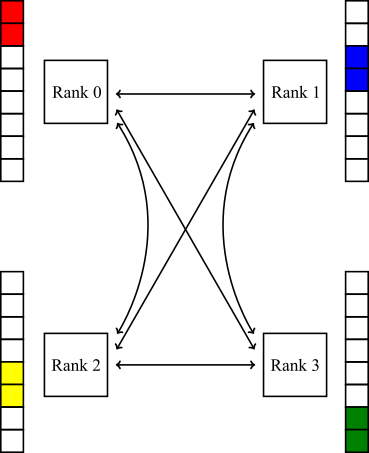
\includegraphics[width=\linewidth]{1acomm.png}
%         \caption{Caption for image 1}
%         \label{fig:1bcomm1}
%     \end{subfigure}
%     \hfill
%     \begin{subfigure}[t]{0.45\textwidth}
%         \centering
%         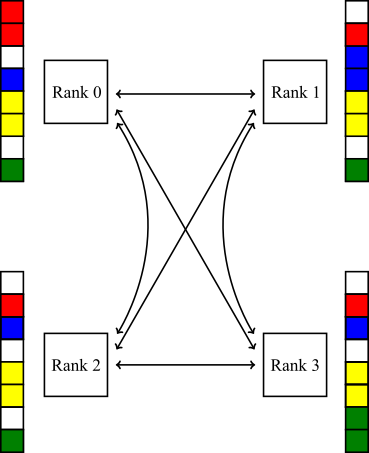
\includegraphics[width=\linewidth]{1bcommdone.png}
%         \caption{Caption for image 2}
%         \label{fig:1bcomm2}
%     \end{subfigure}
%     \caption{Main figure caption describing both subfigures}
%     \label{fig:1bcomm}
% \end{figure}


\section{Strategy C - Exchange only required separators}
Further reduciton to the communication volume can be achieved by observing that not all separator values are required by every process. As the number of partitions increases, the set of dependencies between partitions tends towards sparcity. As a consequence of this, certain sets of separators may only need to be communicated to a given subset of processes. Using this strategy, each process only communicates its set of separator values to the processes that require them. The communication pattern in illustrated in Figure \ref{fig:1ccomm}, and Algorithm \autoref{alg:1ccomm} shows how this can be implemented.

Let \(n_{p}\) be the total number of ranks, \(n_{i}\) be the number of neighbours of rank \(i\), and \(s_{i}\) the size of the separator of rank \(i\). With \(n_{i} \leq n_{p}\), the total communication volume is given by \ref{eq:1ccomm}.

\begin{equation}
    \label{eq:1ccomm}
    \sum_{i=1}^{n_{p}} s_i \cdot  n_{i} 
\end{equation}

\begin{algorithm}[H]
    \label{alg:1ccomm}
    \caption{Exchange only required separators}
    \SetAlgoVlined
    \SetKwInOut{Input}{Input}
    \SetKwInOut{Output}{Output}
    \Input{y, rank,size, displacements, sendItems, sendCount}
    \Output{\newline}

    % mpiRequests \(\gets\) [MPI\_Request] \(\cdot\)  \(2 \cdot \) size\\
    % reqCount \(\gets\) 0\\
    MPI\_Requests \(\gets\) 0\\
 
    \For{r = 0; r < size; r++}{
        \If{rank = r or sendItems[r][rank] = 0}{
            continue\\
        }

        Post non-blocking MPI receive for \(sendCount[r]\) elements at address \(y + displacements[r]\)\\
        MPI\_Requests++\\
    }

    \For{r = 0; r < size; r++}{
    \If{rank = r or sendItems[r][rank] = 0}{
        continue\\
    }
    Post non-blocking MPI send of \(sendCount[rank]\) elements to address \(y + displacements[rank]\)\\
    MPI\_Requests++\\
    }
    Wait for all non-blocking requests to complete\\
\end{algorithm}


\begin{figure}[H]
    \centering
    \incfig{1ccomm}
    \caption{Contents of each ranks \(x\) vector before and after communication under the \textit{Exchange Reuired Separators} communication pattern.}
    \label{fig:1ccomm}
\end{figure}

\section{Strategy D - Exchange only required separator values}
The final strategy further reduces the communication volume by only communicating the separator elements to the rank with which that element induces a data dependency. This approach eliminates all unnecessary data transfers but introduces additional complexity in managing communication schedules. It requires careful management of the send and recieve lists, and introduces some additional overhead by means of a packing and unpacking step necessary for transmitting the data between ranks. This overhead does however not outweigh the benefits gained from the reduction in communication volume which this strategy yields.
\medskip

Both strategy B and C requires reordering of the separator values, in order to make the communication of the separators easier, but due to the packing and unpacking step required for this strategy as seen in algorithm \ref{alg:reqsepexchange}, reordering the separator elements is not required for this communication strategy.
\medskip

Let \(n_{p}\) be the total number of ranks, and let \(d_{i}\) be the number of elements in rank \(i\)s separator that are required by other ranks. Since this communication strategy only communicated these elements, the total communication volume is given by \ref{eq:1dcomm}.

\begin{equation}
    \label{eq:1dcomm}
    \sum_{i=1}^{n_{p}} d_{i} 
\end{equation}

\begin{algorithm}[H]
    \label{alg:reqsepexchange}
    \caption{Strategy D - Packing, exchanging and unpacking separator elements}
    \SetAlgoVlined
    \SetKwInOut{Input}{Input}
    \SetKwInOut{Output}{Output}
    \Input{c, $x$, rank, size}
    \Output{Updated vector $x$}

    totalSend, totalRecv $\gets$ 0\\
    \For{i = 0; i < size; i++}{
        totalSend $\gets$ totalSend + c.sendCount[i]\\
        totalRecv $\gets$ totalRecv + c.receiveCount[i]\\
    }

    Allocate sendBuffer[totalSend], recvBuffer[totalRecv]\\

    sendOffset $\gets$ 0\\
    \For{i = 0; i < size; i++}{
        \For{j = 0; j < c.sendCount[i]; j++}{
            sendBuffer[sendOffset++] $\gets$ $x$[c.sendItems[i][j]]\\
        }
    }

    Compute sendDispls, recvDispls as prefix sums of c.sendCount, c.receiveCount\\

    MPI\_Ialltoallv(sendBuffer, c.sendCount, sendDispls, recvBuffer, c.receiveCount, recvDispls)\\

    MPI\_Waitall()\\

    recvOffset $\gets$ 0\\
    \For{i = 0; i < size; i++}{
        \For{j = 0; j < c.receiveCount[i]; j++}{
            $x$[c.receiveItems[i][j]] $\gets$ recvBuffer[recvOffset++]\\
        }
    }

    Free sendBuffer, recvBuffer, sendDispls, recvDispls\\
\end{algorithm}




\begin{figure}[ht]
    \centering
    \incfig{1dcomm}
    \caption{Contents of each ranks \(x\) vector before and after communication under the \textit{Exchange Reuired Elements} communication pattern.}
    \label{fig:1dcomm}
\end{figure}


\section{Strategy E - Memory Scalable}
\label{sec:memscal}
The communication strategies discussed so far all have a common problem that prevents them from scaling to large matrices. These strategies all store the entire vector \(x\), and will run into performance issues when \(x\) is so large that it doesn't fit into memory. Usually, this is not a problem when SpMV is ran on CPUs, as they have large amounts of memory. Even on GPUs this problem might not be encountered, as modern GPUs have sufficient memory for large matrices.
\medskip

% \Huge{WRITE ABOUT SEPARATOR REORDERING}

Instead of storing the entire vector, each rank only stores its local part of the vector. In addition, it is necessary to allocate enough space for the separators elements that are needed from the other ranks. In order to achieve this, \(x\) is renumbered such that every ranks part of the vector is 0-indexed. For the local part of the \(x\) vector this is done by simply subtracting the position of the first local entry assigned to that rank from each entry in the local vector. It is also necessary to reorder the separator elements, as they will be stored after the entries in the local vector. This is achieved in a similar manner as the algorithm outlined in \ref{alg:reorderseparators}.

% It is slightly more complicated to renumber the separator elements, and the technicalities of how to do this will not be discussed here.
\medskip


% There is no specific communication pattern that are required for 

\begin{figure}[ht]
    \centering
    \incfig{2dcomm}
    \caption{Global indexing vs. Local indexing of \(x\).}
    \label{fig:2dcomm}
\end{figure}








